\documentclass[11pt,twoside]{article}

\usepackage[margin=2cm]{geometry}
\usepackage{tikz}
\usetikzlibrary{positioning,fit,shapes}

\newcommand{\name}[1]{ {\color{red}{\sffamily\bfseries{#1}}} }

\title{NewActon design}
\author{Mengyan Zhang}
\date{04 October 2018}

\begin{document}
\maketitle

\section*{NewActon}

Recommenders, predictors, and labellers are stateful "agents": only they can access their own internal state; other agents should ask them directly. Each agent stores their state in its own file. In this case, the whole system can be rebooted from any point with low coupling.  
 
 \begin{figure}[h]
     \centering
     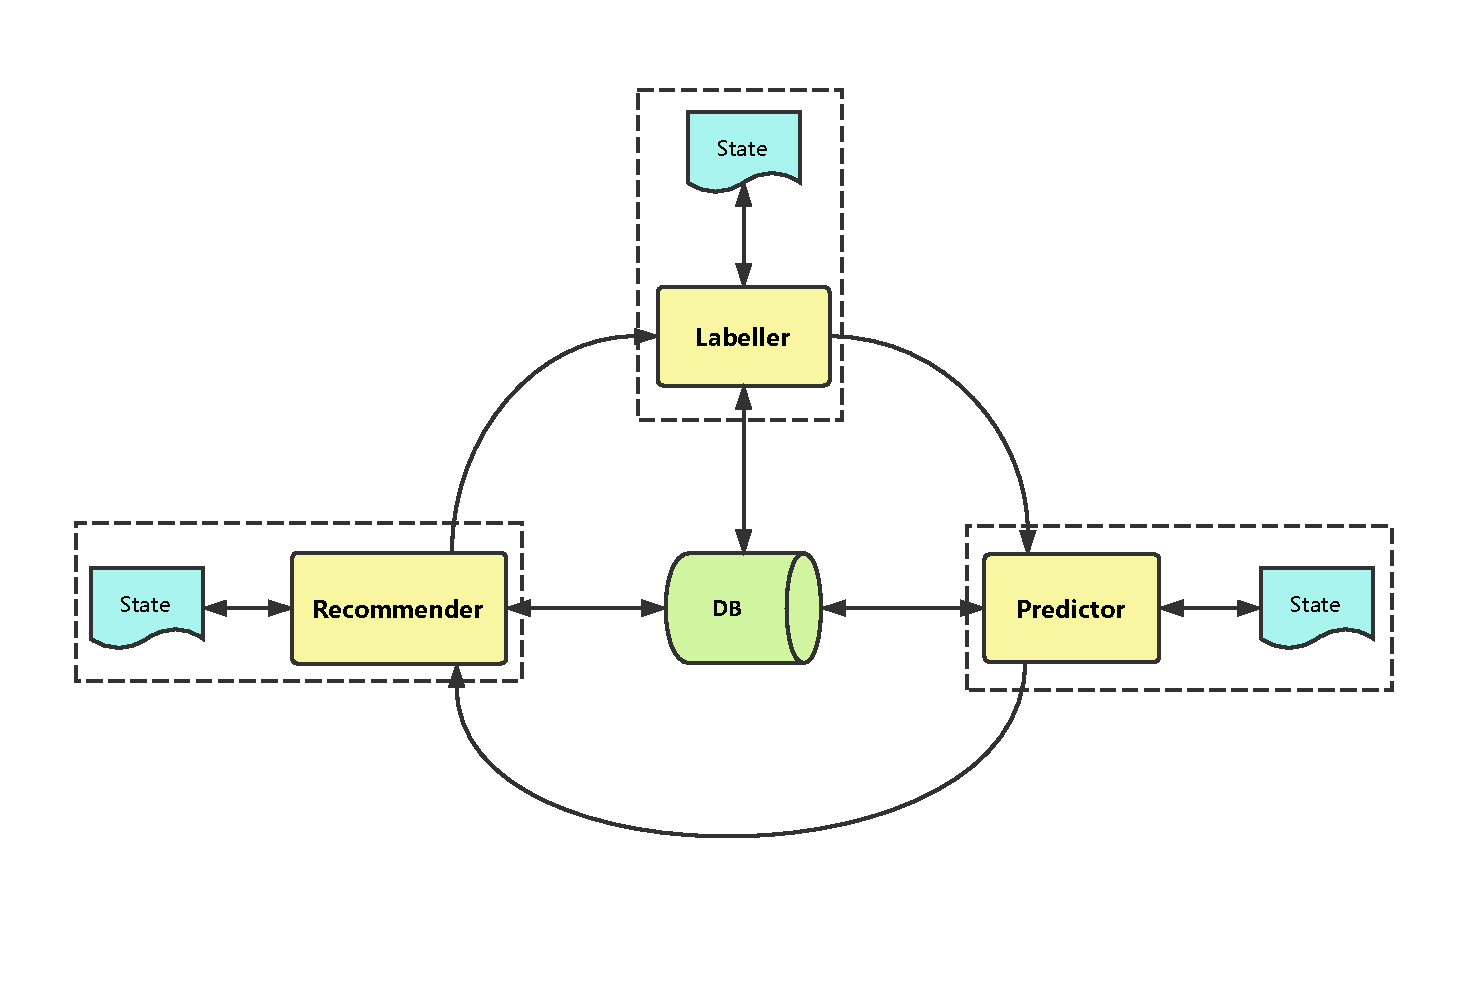
\includegraphics[scale = 0.7]{docs/design/acton.pdf}
     \caption{NewActon Design Choice}
     \label{fig:my_label}
 \end{figure}

\subsection*{What's in state file?}

Labeller: observed labels \newline
Predictor: latest prediction \newline   
Recommender: recommendations

\subsection*{What should be passed?}

Labeller $\rightarrow$ Predictor: observed labels \newline
Predictor $\rightarrow$ Recommender: prediction array (matrix) \newline
Recommender $\rightarrow$ Labeller: recommendations \newline
What should be passed over is exactly the information should be recorded in the state file.

\subsection*{Graph Extension}

A graph model contains nodes and edges, where nodes represent entities (e.g. person) and edges represent relations (e.g. friendship). We use a three-way tensor $\mathcal{X} \in \{0,1\}^{K \times N \times N}$ to represent the graph model, where K is the number of relations and N is the number of entities, and $x_{ikj}$ indicates whether the triple is valid.\newline
To recommend as many valid triples to get labels as possible, we use Thompson Sampling model to predict the probability of a triple being valid and recommend the triple with the highest probability. \newline
\newline
Labeller: the same as before. \newline
Recommender: Thompson sampling, recommends triple (i,k,j) = {argmax}$_{i,k,j} P(x_{ikj})$ \newline
Predictor: update posterior distribution based on Bayesian inference; sample latent variables from the posterior distribution.


\end{document}
